\documentclass{beamer}
\usepackage[utf8]{inputenc}
\usepackage[english,russian]{babel}
\usepackage{hyperref}
\usepackage{xcolor}
\usepackage{graphicx}

\usetheme{Boadilla}
\usecolortheme{seahorse}
\setbeamercovered{transparent}% Allow for shaded (transparent) covered items

\AtBeginSection[]
{
  \begin{frame}
    \frametitle{Содержание}
    \tableofcontents[currentsection]
  \end{frame}
}

\begin{document}

\title[]{Git: распределённая система контроля версий}
\author{Н.\,Д.~Кудасов}
\institute{МГУ им. Ломоносова}
\date{Москва, 2013}

\begin{frame}
\addtocounter{framenumber}{-1}
\maketitle
\end{frame}

\section{Введение}

\begin{frame}
  \frametitle{Системы контроля версий}

  Системы контроля версий позволяют отслеживать изменения в коде, документах и пр.

  \begin{block}{Централизованные системы}
  Единый сервер для хранения документов и истории.
  Централизованный контроль над хранилищем.
  \end{block}

  \begin{block}{Распределенные системы}
  Каждый пользователь имеет собственную версию репозитория.
  Изменение могут передаваться между репозиториями.
  \end{block}
\end{frame}

\begin{frame}
  \frametitle{Зачем нужны системы контроля версий?}
  Случалось ли, что Вы
  \begin{itemize}
    \item изменили код, обнаружили ошибку и захотели откатиться?
    \item потеряли код, а имеющийся бекап оказался устаревшим?
    \item должны были поддерживать несколько версий программы?
    \item хотели посмотреть, чем отличаются две версии программы?
    \item хотели обнаружить, какое изменение внесло ошибку в программу?
    \item хотели просмотреть историю исходного кода?
    \item хотели отправить изменение для чужого кода?
    \item хотели выложить код, чтобы другие могли работать над ним?
    \item хотели посмотреть, сколько работы проделано? Когда? Кем?
    \item хотели попробовать что-то новое, не ломая основного кода?
    \item и т.д.
  \end{itemize}
\end{frame}

\begin{frame}
  \frametitle{Системы контроля версий: примеры}
  \begin{block}{Централизованные системы}
    \begin{itemize}
      \item CVS
      \item Subversion (SVN)
      \item Visual SourceSafe, Vault и т.д.
    \end{itemize}
  \end{block}

  \begin{block}{Распределенные системы}
    \begin{itemize}
      \item Git,
      \item Darcs,
      \item Mercurial, Bazaar,
      \item Bitkeeper и т.д.
    \end{itemize}
  \end{block}
\end{frame}

\begin{frame}
  \frametitle{Git}
  Одна из наиболее популярных систем контроля версий.

  \begin{block}{Основные преимущества}
    \begin{itemize}
      \item пример хорошо написанной и производительной программы на C;
      \item компактный репозиторий (эффективное сжатие и хранение истории);
      \item множество копий/бекапов;
      \item произвольная организация работы с несколькими репозиториями;
      \item промежуточная область для коммитов;
      \item простые в использовании ветки.
    \end{itemize}
  \end{block}
\end{frame}

\begin{frame}
  \frametitle{Git: проекты}
  Git подходит для использования в любом проекте (как и любая
  распределенная система контроля версий).

  \begin{block}{Примеры использований}
    \begin{itemize}
      \item ядро ОС Linux и смежные проекты;
      \item gcc и смежные проекты;
      \item ОС Android,
      \item Qt, Cairo,
      \item Ruby on Rails, jQuery,
      \item GitHub.com,
      \item огромное количество других проектов.
    \end{itemize}
  \end{block}
\end{frame}

\section{Git: модель репозитория}

\begin{frame}
  \frametitle{Основы}
  Git хранит информацию о проекте и его истории в специальной структуре,
  которая называется {\it репозиторий}. Помимо прочего, репозиторий включает
  в себя набор {\it коммитов (commit objects)} и {\it ссылок на коммиты (heads)}.

  \begin{block}{Коммит}
    \begin{itemize}
      \item набор файлов, соответствующий состоянию проекта на заданный момент времени;
      \item ссылки на родительские коммиты;
      \item уникальный SHA1-код (хеш), однозначно идентифицирующий коммит.
    \end{itemize}
  \end{block}

  \begin{block}{Ссылки}
    \begin{itemize}
      \item просто ссылка на коммит;
      \item ссылки имеют имена, по умолчанию создается ссылка {\it master};
      \item ссылка, активная на текущий момент, имеет синоним {\it HEAD}.
    \end{itemize}
  \end{block}
\end{frame}

\begin{frame}
  \frametitle{Первоначальная настройка}
  Прежде, чем начать работать с Git, ему необходимо сообщить немного о себе:

  \begin{figure}
     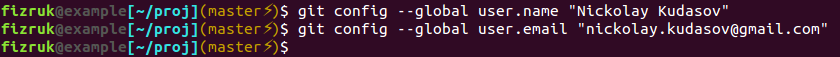
\includegraphics[width=12cm]{images/git-config.png}
  \end{figure}

  Эта информация будет использована в истории, чтобы можно было проследить,
  кто отвественен за какие изменения.

  Опция \texttt{--global} вносит изменения в файл \texttt{.gitconfig} в
  домашней директории. Этот файл используется по умолчанию. Если опция
  не указана, настройки применяются только к текущему репозиторию.
\end{frame}

\begin{frame}
  \frametitle{Создание репозитория}
  При создании репозитория, Git создаёт служебную директорию \texttt{.git/}
  в корне проекта:
  \begin{figure}
     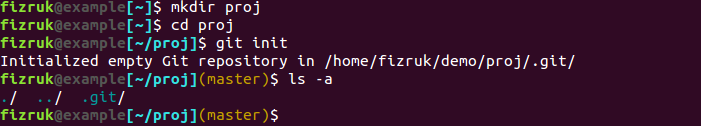
\includegraphics[width=10cm]{images/git-init.png}
  \end{figure}

  Команда \texttt{git add} регистрирует изменения, которые попадут в очередной коммит.
  Команда \texttt{git commit} создаёт коммит.

  \begin{figure}
     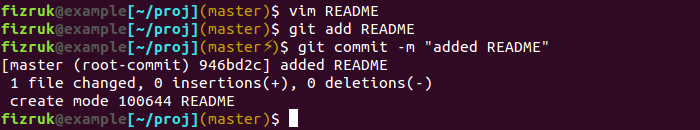
\includegraphics[width=10cm]{images/git-add-commit.png}
  \end{figure}

  Этих команд уже хватает для работы над проектом с Git!
\end{frame}

\begin{frame}
  \frametitle{Просмотр истории}
  Команда \texttt{git log} позволяет показать историю изменений:

  \begin{figure}
     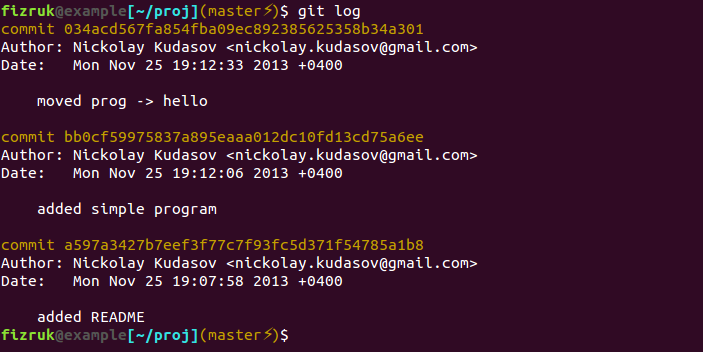
\includegraphics[width=10cm]{images/git-log.png}
  \end{figure}

  \begin{figure}
     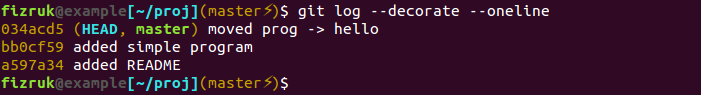
\includegraphics[width=10cm]{images/git-log-oneline-decorate.png}
  \end{figure}
\end{frame}

\begin{frame}
  \frametitle{Состояние проекта}
  Команда \texttt{git status} позволяет посмотреть список изменений
  (зарегистрированных, незарегистрированных, новых файлов, и т.д.):

  \begin{figure}
    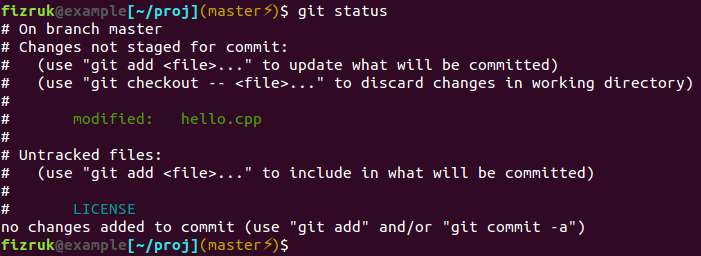
\includegraphics[width=10cm]{images/git-status.png}
  \end{figure}
\end{frame}

\begin{frame}
  \frametitle{Просмотр изменений}
  Команда \texttt{git diff} позволяет посмотреть сами изменения:

  \begin{figure}
    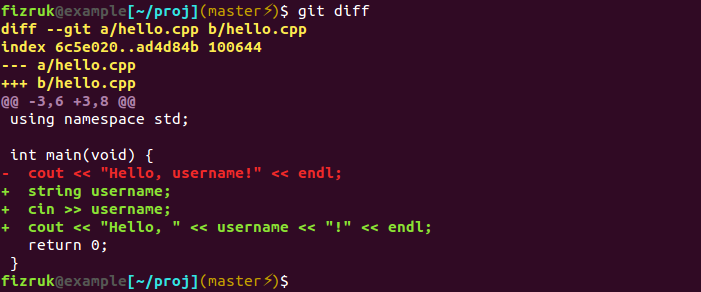
\includegraphics[width=10cm]{images/git-diff.png}
  \end{figure}
\end{frame}

\section{Git: основные операции}

\section{GitHub: открытое взаимодействие}

\end{document}

